\begin{chapter}{Estado de la tecnología}
\label{chap:estado-tecnologia}
    \lettrine{C}{on} el desarrollo de las tecnologías web y la comercialización por parte de grandes empresas de su infraestructura, los servicios \textit{Infrastructure as a Service} (IaaS) han ganado una popularidad considerable, con ello también se han desarrollado herramientas software dedicadas a la gestión de infraestructura para la implementación de sistemas Cloud Computing. Algunas de estas son VMware Cloud Foundation (creado en 2011), OpenStack (creado en 2010) o Apache CloudStack (creado en 2012). Estos productos proveen software que permite construir una infraestructura virtualizada sobre un conjunto de recursos físicos, con el objetivo de separar la administración de la capa física de la capa virtual para simplificar y automatizar la gestión y escalabilidad de los recursos. Proponen un modelo que persigue reducir costes de gestión de la infraestructura y aumentar la disponibilidad del servicio, es decir, aumentar la eficiencia de la infraestructura física.
    A lo largo de este capítulo se expone la solución Cloud propuesta para ser implementada en la infraestructura del CITIC indicando las razones de su elección y sus principales características.

\begin{section}{Servicio Cloud}    
    Como ya se ha visto, en el mercado existen varias alternativas que se pueden utilizar para cumplir los objetivos del proyecto. Finalmente, se ha escogido el producto \textbf{VMware Cloud Foundation} (VCF) ya que al pertenecer al mismo proveedor que el software de virtualización empleado en la infraestructura del CITIC, todos sus componentes se integran perfectamente con los componentes de VMware ya instalados en la infraestructura, por lo tanto, su mantenimiento es más sencillo y su funcionamiento más eficiente. También es posible integrar soluciones de otras compañías pero, al estar fuera del ecosistema de VMware podrían producirse problemas de compatibilidad entre versiones a largo plazo con los productos existentes en la infraestructura del CITIC. Utilizando los productos de un mismo proveedor se asegura el soporte del software instalado y la obtención del máximo rendimiento de cada componente.        
    \begin{subsection}{VMware Cloud Foundation}
    
        Esta solución de VMware virtualiza todas las capas de la infraestructura combinando cuatro de sus productos. Utiliza \textbf{VMware vSphere} para virtualizar y gestionar el cómputo, \textbf{VMware vSAN} para virtualizar y gestionar el almacenamiento, \textbf{VMware NSX-T} para la virtualización y gestión de la red, y \textbf{VMware vRealize Suite} para gestionar las operaciones de la infraestructura virtual como el aprovisionamiento de recursos. Todos estos servicios juntos convierten el CPD en un Software Defined Datacenter (SDDC), un entorno donde existe una infraestructura física abstraída en una capa virtual separando así la gestión de ambas. Esto permite modificar la infraestructura virtual según se requiera sin necesidad de modificar la configuración de la infraestructura física, favoreciendo la automatización y dinamismo de tareas y la elasticidad de los recursos. Gracias a esto, con VCF es posible habilitar el aprovisionamiento de recursos por parte de los usuarios para ofrecer así un servicio de IaaS. Con esta solución se obtienen las siguientes características:
        
    \begin{itemize}
        \item Servicios software con integración nativa: ofrece un conjunto de servicios software para el almacenamiento, red, seguridad y gestión del servicio Cloud. Estos servicios se integran de forma nativa con la infraestructura minimizando las tareas de configuración y administración.
        \item Escalabilidad y elasticidad de los recursos: la capacidad de la infraestructura se puede modificar de forma sencilla gracias a la automatización del ciclo de vida de todos los elementos y al desacople entre las dos capas (la física y la virtual).
        \item Supervisión de los recursos: monitoriza los recursos con reconocimiento de aplicaciones y solución de problemas, permitiendo conocer todos los eventos que tienen lugar en la infraestructura. También permite establecer políticas de seguridad en cuanto al acceso a los recursos y la red.
        \item Aprovisionamiento automatizado: permite la obtención de recursos de forma automática incluyendo servicios de red, almacenamiento y cómputo. Los componentes de la infraestructura virtualizada se encargan de la reserva de los recursos y de todas las operaciones necesarias para llevarla acabo.
    
        \item Ciclo de vida automatizado: automatiza las operaciones de gestión previas, iniciales y posteriores de la plataforma para simplificar y coordinar su gestión. En estas tareas incluye el despliegue de la plataforma y su implementación, la escalabilidad de los recursos físicos y la instalación de actualizaciones para cada componente software.
    
    \end{itemize}
    \begin{figure}[h!]
        \centering
        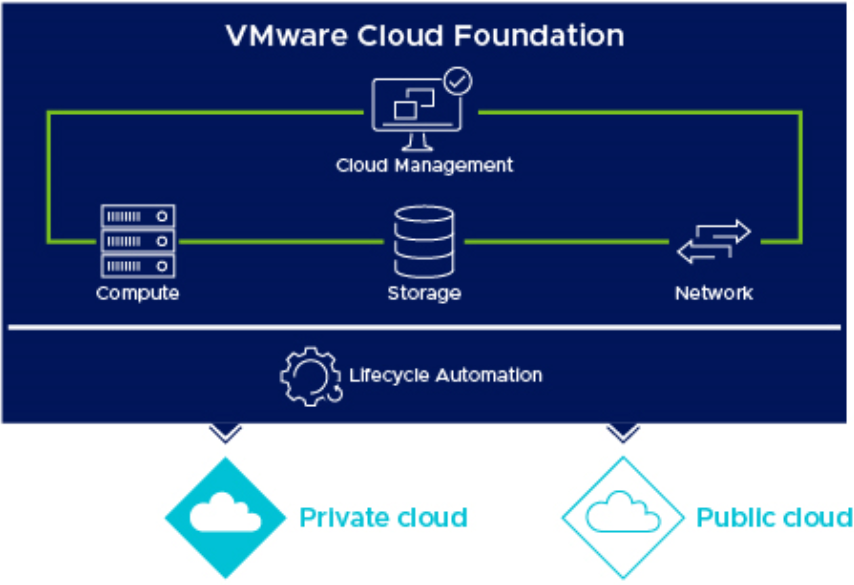
\includegraphics[width=0.6\textwidth]{imaxes/cap2recursos/overviewCF.png}
                \caption{Estructura de VMare Cloud Foundation.}
        \label{fig:Cloud-Foundation-Overview}
        \end{figure}
        \FloatBarrier
        \begin{figure}[h]
            \centering
            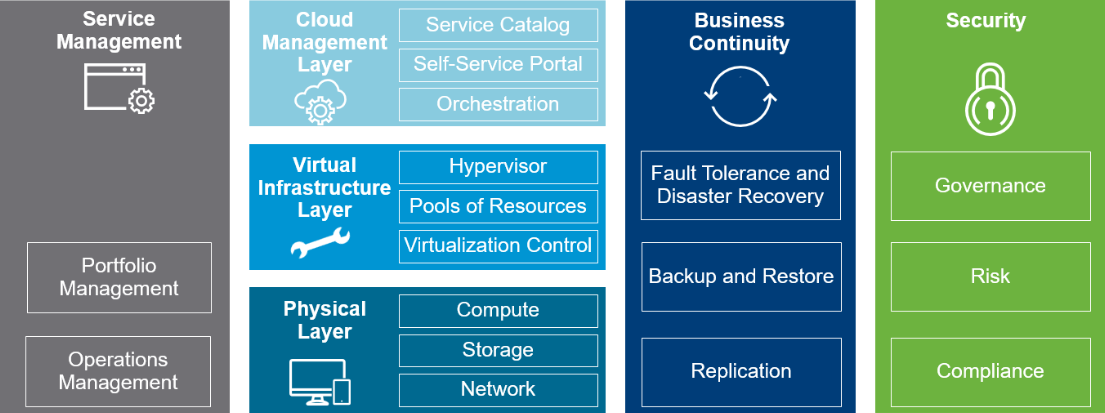
\includegraphics[width=0.8\textwidth]{imaxes/cap2recursos/SDDCoverview.png}
            \caption{Elementos de un SDDC gestionado con VMware Cloud Foundation.}
            \label{fig:layers-Sddc}
        \end{figure}
        \FloatBarrier
    \end{subsection}
    
    \begin{subsection}{Componentes de VMware Cloud Foundation}
    \label{subsubsect:cfcomponents}
    
    Ya se ha visto que VCF está formado por cuatro productos principales. En este apartado se describirán las características de esos cuatro componentes más el servicio que los coordina\footnote{Las características del componente VMware vSphere son las mismas que las descritas en el punto \ref{subsec:softwareinstalado}}. Se utilizará la versión 4.0 de VMware Cloud Foundation lo cual implica que se implementarán las versiones\cite{componentesCloudFound} 4.0 de SDDC Manager, 7.0.0 de VMware vSphere, 7.0.0 de VMware vSAN, 3.0 de VMware NSX-T y 8.2 de VMware vRealize Suite.
    \begin{figure}[h]
        \centering
            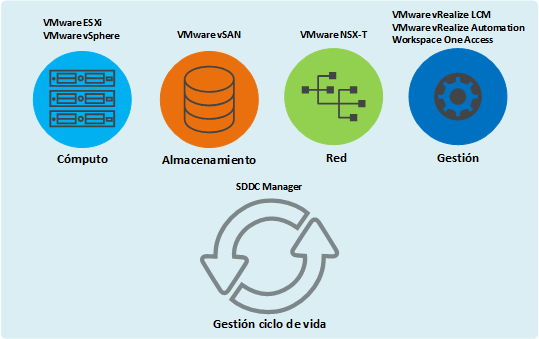
\includegraphics[width=0.6\textwidth]{imaxes/VCF-componentes/ComponentesVCF.png}
            \caption{Partes de un SDDC y componentes de VCF que las implementan.}
            \label{fig:componentes-funciones-VCF}
        \end{figure}
        \FloatBarrier
    \begin{subsubsection}{SDDC Manager}
        SDDC Manager se encarga de gestionar el ciclo de vida de todos los componentes de VCF, esto incluye el despliegue de cada uno, su configuración y la obtención e instalación de actualizaciones. Centraliza la gestión de las licencias y certificados de cada componente y administra el aprovisionamiento de nuevos recursos físicos para el SDDC y los ya existentes.
    \end{subsubsection}
    
    \begin{subsubsection}{VMware vSAN}
        VMware vSAN virtualiza el almacenamiento del SDDC. Permite gestionar de forma centralizada, el sistema de almacenamiento sin necesidad de tener que modificar la configuración física. El sistema de almacenamiento se abstrae para formar único datastore sobre el que se establecen políticas de uso y disponibilidad. El acceso por parte de cada host al datastore se realiza mediante el protocolo IP, a través de una subred dedicada al servicio. El datastore está formado por discos de almacenamiento que se organizan en grupos que se asignan a un host. Los grupos pueden tener configuración \textit{Hybrid}, que combina discos HDD y SDD, o configuración \textit{All-Flash} que solo utiliza SSD y por lo tanto tiene mayor rendimiento. Dentro de cada grupo existe un disco de caché y al menos un disco de capacidad donde se almacenan los datos persistentes\cite{operacionesVSAN}. 
        % En el modo \textit{All-Flash}\footnote{Solo se describe el modo \textit{All-Flash} porque es la configuración recomendada por VMware.} la operación de lectura se realiza directamente sobre los discos de capacidad y la operación de escritura se hace sobre el disco caché que posteriormente escribe los datos en el disco de capacidad.
        
        \begin{figure}[h]
        \centering
            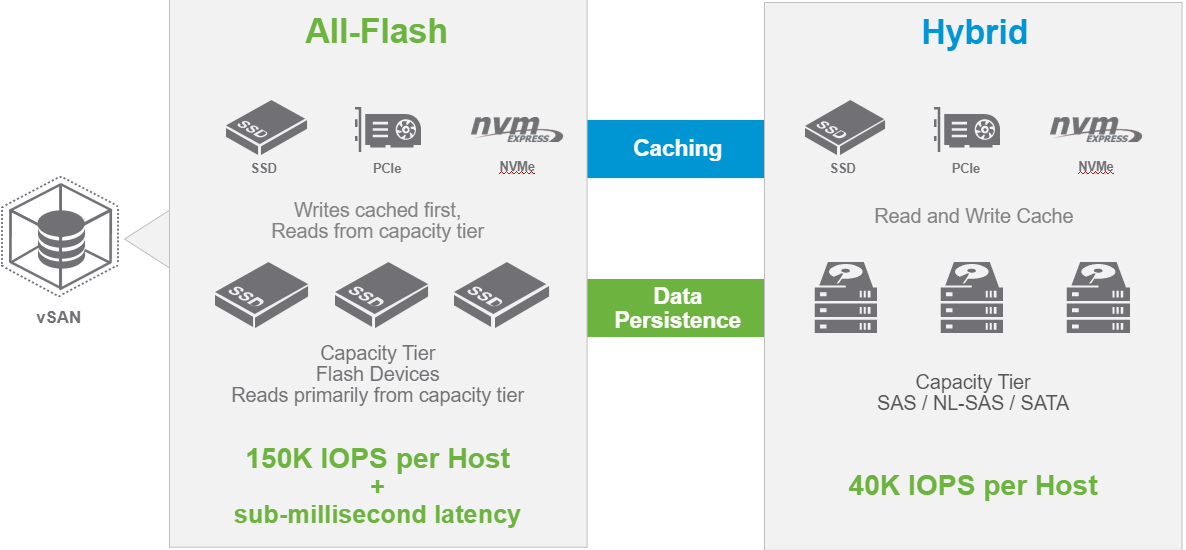
\includegraphics[width=0.6\textwidth]{imaxes/cap2recursos/rendimientoVSAN.png}
            \caption{Configuración \textit{All-Flash} y configuración \textit{Hybrid} en vSAN.}
            \label{fig:performance-Hybrid-AllFlash-vSAN}
        \end{figure}
        \FloatBarrier
    \end{subsubsection}
    
    \begin{subsubsection}{VMware NSX-T}
        VMware NSX-T virtualiza la red del SDDC. Abstrae los componentes físicos de la red para generar una red virtual desacoplada de la infraestructura física, esta se configura sin modificar la red física y para ello aporta servicios de red virtualizados y la posibilidad de crear y extender subredes sobre la infraestructura. Internamente tiene tres componentes, NSX-T Manager, NSX-T Controller y NSX-T Edge. El primero, es el punto de acceso a la configuración de VMware NSX-T y el que almacena y transmite la configuración establecida, el segundo controla las redes y se encarga de informar sobre el estado y la configuración de las redes virtuales. El último componente, NSX-T Edge, proporciona servicios de red y enrutamiento a las redes virtuales. Los hosts integrados en VMware NSX-T se encargan de controlar el tráfico y monitorizar la infraestructura virtual creada por VMware NSX-T.
        % El control del tráfico y la monitorización de las conexiones se hace desde el componente \textbf{Transport Node} (TN) con la información que recibe de las instancias de NSX-T Controller. Existen dos tipos de TNs, \textbf{Hypervisor Transport Node} que son hosts con ESXi instalado y que están configurados para correr los servicios de VMware NSX-T, y \textbf{NSX-T Edge Node} que se trata de una \textit{appliance} instalada en una VM o sobre un host físico para proveer un conjunto de servicios de red centralizados para las redes virtuales de VMware NSX-T.
        \begin{figure}[h!]
            \centering
                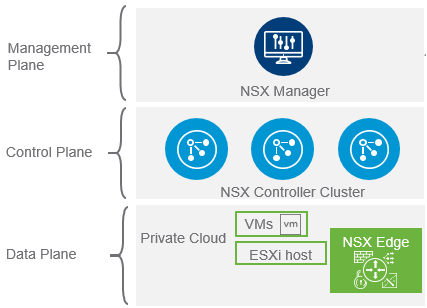
\includegraphics[width=0.6\textwidth]{imaxes/VCF-componentes/nsx-t-layers.png}
                \caption{Componentes de VMware NSX-T y capas en las que se dividen.}
                \label{fig:nsx-t-components}
            \end{figure}
            \FloatBarrier
    \end{subsubsection}
    
    \begin{subsubsection}{VMware vRealize Suite}
        VMware vRealize Suite agrupa un conjunto de productos que si bien no son obligatorios para desplegar VCF, aportan funcionalidades extra que completan la formación del SDDC. Los productos que se utilizarán en este proyecto son \textbf{vRealize Suite Lifecycle Manager} dedicado a gestionar el despliegue, actualizaciones, certificados y licencias de los productos que forman VMware vRealize, \textbf{Workspace One Access} dedicado a gestionar los usuarios y ser el punto de acceso centralizado de las aplicaciones de VMware vRealize Suite y, finalmente, \textbf{vRealize Automation} el cual permite a los usuarios del SDDC diseñar y aprovisionar un conjunto de recursos de la infraestructura según sus necesidades y de forma automatizada mientras el administrador puede limitar la cantidad de recursos que se consumen.
    \end{subsubsection}
    \end{subsection}

    \begin{subsection}{Conceptos}
        En este apartado se describen algunos conceptos que se deben tener claros para entender la estructura y arquitectura de los componentes de VCF.
        % En este apartado se describe la arquitectura de VMware Cloud Foundation y como estructura sus componentes\footnote{Se describen solo aquellos componentes que se utilizarán en el despliegue de Cloud Foundation.} internamente.
        
        %%%%%%%%%%%%%%%%%%%%%%%%%%%%%%
        % \iffalse
        % En este apartado se explican aquellos conceptos de VMware Cloud Foundation necesarios para entender su funcionamiento, configuración y requisitos de la infraestructura previos al despliegue del servicio.
        % \fi
        %%%%%%%%%%%%%%%%%%%%%%%%%%%%%%%%
        
        
        %% Workload Ddomains %&%&%%%%
        %%%%%%%%%%%%%%%%%%%%%%%%%%%%
        \begin{subsubsection}{Workload Domain}
        Un Workload Domain (WD) representa un bloque de recursos dentro del SDDC, formado por recursos físicos y virtuales y gestionados por los componentes de VCF. En cada WD se despliegan instancias de los componentes de VCF para controlar el acceso y uso de los recursos, estableciendo, además, una capa de seguridad sobre el WD. Esto permite que los recursos de cada WD se gestionen de forma separada. La función de un WD consiste en separar flujos de trabajo para determinar que recursos se dedican a la realización de determinadas tareas.
        \end{subsubsection}
        %% MANAGEMENT DOMAIN
        \begin{subsubsection}{Management Domain}
        \label{subsubsec:domainManagement}
        El Management Domain es el primer WD que se crea dentro del SDDC cuando se despliega VCF. Su finalidad es alojar todos los componentes de VCF que gestionan el propio Management Domain y al resto de WDs por lo tanto todas las tareas de administración de la infraestructura están centralizadas dentro de este WD. Inicialmente, se despliegan las siguientes VMs de cada componente:
        \begin{itemize}
          \item Una VM de SDDC Manager.
          \item Una VM de VMware vCenter Server.
          \item Tres VMs de VMware NSX-T Manager.
          \item Dos VMs de VMware NSX-T Edge.
        \end{itemize}
        % Al contener todas las instancias de los componentes dedicados a la gestión del SDDC, todas las tareas de administración suceden dentro de este WD. De esta forma, su ejecución está centralizada, es más segura y está mejor controlada, ya que lo hacen sobre un conjunto de recursos dedicados exclusivamente a ellas.
        \end{subsubsection}        
        %% VIRTUAL INF. DOMAIN
        \begin{subsubsection}{Virtual Infrastructure Domain (VI)}
        \label{subsubsec:domainVI}
        Este tipo de WD se crea manualmente y bajo demanda desde el Management Domain, para habilitar un entorno cuyos recursos puedan ser usados por los usuarios mediante el despliegue de aplicaciones. Su objetivo es separar las tareas y recursos dedicados a la administración del SDDC de las tareas y recursos utilizados por los usuarios del servicio. Con la creación de un WD se generan las siguientes VMs:
        \begin{itemize}
            \item Una VM de VMware vCenter Server que se sitúa en el Management Domain.
            \item Tres VMs de VMware NSX-T Manager situadas en el Management Domain.
            \item Dos VMs de VMware NSX-T Edge.
          \end{itemize}
        % Su configuración de hardware y lógica se especifican durante el proceso de creación, pudiendo establecer la cantidad de hosts, cantidad de almacenamiento, configuración de la red y políticas de rendimiento y disponibilidad, todo para satisfacer las necesidades del tipo de tareas que se van a realizar en él. 

        % Que ciertos componentes se sitúen en el Management Domain, permite separar las tareas de administración de un VI Domain de las aplicaciones y recursos de los usuarios, haciendo un entorno mejor organizado, más seguro y óptimo.
         \end{subsubsection}

        %&%%%%%%%%%%%%%%%%%%%%%%%%%%%%%%%%%%%%%%%%%%%%%%%%%%%%%%%%
        %% ARQUITECTURA
              
        % \begin{subsection}{Arquitectura}
        % VMware proporciona dos posibles modelos de arquitectura diferentes. Se utiliza uno u otro dependiendo del tamaño de la infraestructura sobre la que se va a desplegar VCF, y con cada modelo, se determina la forma en la que se agruparán y administrarán los recursos del SDDC.
        
        %%%%%%%%%%%%%%%%%%%%%
        %%%%%%%%%%%%%%%%%%%%%%%%
        %% ESTANDAR
        \begin{subsubsection}{Modelo de arquitectura estándar}
        Este modelo está pensado para entornos de tamaño medio/grande, con un mínimo de siete hosts. Está formado por un Management Domain y al menos un VI Domain. Esto implica que la ejecución de tareas dentro de un WD está limitada por los recursos que lo forman. Esto permite asignar roles a los recursos según las operaciones que se van a ejecutar sobre ellos, establecer un nivel de seguridad en cada WD y dedicar un conjunto de recursos a la ejecución de cierto tipo de operaciones. Así, el entorno es más eficiente, ya que se proporciona una forma de adecuar la configuración de los recursos de acuerdo con el uso que se va a hacer del servicio o servicios desplegados, minimizando además los cambios sobre la infraestructura física.
        \begin{figure}[h!]
          \centering
          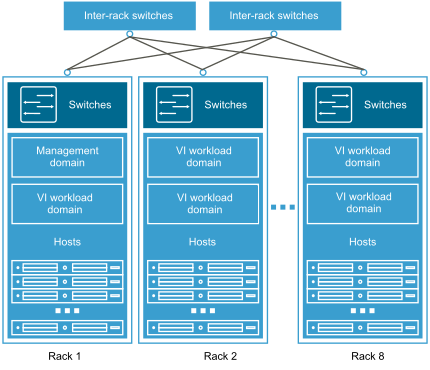
\includegraphics[width=0.6\textwidth]{imaxes/conceptosPrevios/arquitect_standarCF.png}
          \caption{Esquema del modelo de arquitectura estándar.}
          \label{fig:modelostandard}
        \end{figure}
        \FloatBarrier
        %%%%%%%%%%%%%%%%%%%%%
        %%  CONSOLIDADO
        \end{subsubsection}
        \begin{subsubsection}{Modelo de arquitectura consolidado}
        Este modelo está orientado a entornos de tamaño pequeño, con menos de siete hosts. Está formado por un único WD que cumple las funciones de un Management Domain y de un VI Domain, es decir, en él se colocan las instancias de los componentes dedicados a la gestión del SDDC\footnote{Se despliega la misma cantidad de instancias de cada componente que en el Management Domain.} junto con las aplicaciones desplegadas para la realización de otro tipo de tareas. Así, a diferencia del modelo estándar, todas las operaciones se ejecutan dentro de un mismo entorno y sobre los mismos recursos. Internamente, las VMs se pueden colocar dentro de grupos, llamados resource pools, en el que se puede establecer un límite de uso de recursos. Este modelo no aporta tantos beneficios como el modelo estándar, ya que todas las operaciones se realizan sobre los mismos recursos, y los niveles de control y seguridad son menores.       
        \begin{figure}[h!]
          \centering
          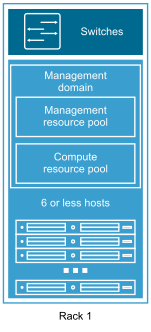
\includegraphics[width=0.25\textwidth]{imaxes/conceptosPrevios/modelConsolidated.png}
          \caption{Esquema del modelo de arquitectura consolidado.}
          \label{fig:modeloconsolidated}
        \end{figure}        
        \end{subsubsection}
        \end{subsection}
        
        \begin{subsubsection}{Distribución de los recursos del SDDC}
          Los recursos de un SDDC pueden estar distribuidos en diferentes localizaciones físicas para proporcionar mayor disponibilidad y recuperación ante fallos. A continuación se enumeran las formas de agrupar los recursos según su ubicación.
        %   se agrupan para formar una estructura que permite usar y gestionar los recursos disponibles de forma conjunta y dinámica.        
        \begin{itemize}
          \item Availability Zone (AZ): se llama AZ a un conjunto de recursos físicos que forman una infraestructura independiente, es decir, cada una tiene su propia fuente de energía, su sistema de refrigeración, su sistema de seguridad y su red, no compartidos con otra AZ, para evitar la propagación de fallos hacia otras AZs. Cuando existen varias AZs, se pueden usar de forma que cuando ocurre un fallo en una de ellas la carga de trabajo se distribuye a una segunda AZ minimizando el tiempo de caída del servicio. Dentro de una AZ se alojan uno o más WDs.
          \item Region: se llama Region a un conjunto de AZs situadas en una misma ubicación, es decir, las AZs de una Region están situadas próximas entre sí. Estas AZs deben tener al menos una latencia de 5 ms\cite{latency} entre ellas. Dentro de un SDDC pueden existir varias Regions pero estas se sitúan en ubicaciones más distantes, la latencia debe ser de al menos 150 ms\cite{latency}. Esta estructura permite ofrecer los servicios de un SDDC en diferentes ubicaciones a la vez que se aumenta su disponibilidad y recuperación ante fallos.    
          \item Cluster: un cluster de VMware vSphere es una agrupación de hosts. A las VMs desplegadas sobre ellos se les aplica una configuración de disponibilidad con los servicios vMotion, vSphere HA y vSphere DRS del componente VMware vSphere, permitiendo determinar como se restablecen las instancias cuando ocurre un fallo dentro del cluster. Un cluster se sitúa dentro de un WD, por lo tanto, sus recursos estarán limitados por el alcance del WD.
        \end{itemize} 
        \begin{figure}[h!]
          \centering
          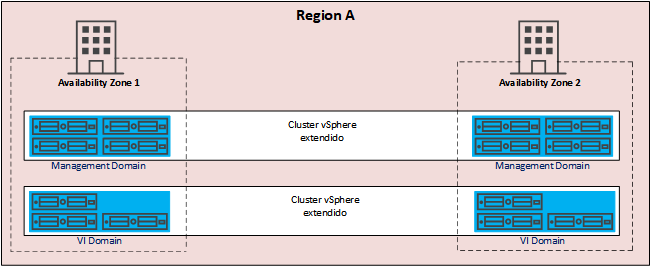
\includegraphics[width=0.8\textwidth]{imaxes/conceptosPrevios/AZRegionCluster.png}
          \caption{Ejemplo de un SDDC con dos Regions y una AZ en cada uno.}
          \label{fig:az-region-cluster}
        \end{figure}
        En la figura anterior se describe el esquema de un SDDC compuesto de una Region. Dentro de esta, existen dos AZ, AZ1 y AZ2. Cada una de las AZs contiene dos WD, un Management Domain desde donde se administra el SDDC, y un VI Domain donde se realizan las operaciones del SDDC. Como se mencionaba anteriormente, las VMs situadas en una AZ pueden migrar de una ubicación a otra en caso de fallo de los recursos físicos. Para ello, el WD donde se encuentran esas instancias debe estar extendido en las dos AZs. En la imagen, el Management Domain está formado por ocho hosts, repartidos en las AZs, los cuales están agrupados dentro del mismo cluster de VMware vSphere, por lo tanto, los componentes cuyas instancias estén situadas en este cluster se podrán migrar entre los 8 hosts. Estas migraciones se realizan en función de la configuración de disponibilidad establecida en los componentes VMware vSphere y VMware vSAN. Así, cuando los hosts de AZ1 sufren una caída, la AZ2 seguiría activa y las instancias situadas en AZ1 migrarían a AZ2 para continuar la disponibilidad del servicio, todo esto de forma automatizada, dinámica y transparente para el usuario. Lo mismo sucedería con el VI Domain\footnote{Se puede encontrar una descripción más detallada de esta estructura en el siguiente enlace \url{https://docs.vmware.com/en/VMware-Validated-Design/6.0/introducing-vmware-validated-design/GUID-661B1CE3-1F74-4E00-80F3-0F5EA39528CD.html}}.
        \end{subsubsection}
    % \end{subsection}
    
    \begin{subsection}{Costes de implementación}
        Los principales costes a la hora de implementar VMware Cloud Foundation en la infraestructura de producción del CITIC son aquellos relacionados con la adquisición de licencias y soporte de los productos. Cada componente de VMware Cloud Foundation requiere su propia licencia\cite{licenses}. El precio de cada licencia dependerá del número de CPUs físicas sobre las que se va usar esta plataforma. Como en la infraestructura hay un total de ocho hosts con dos CPUs cada uno, \underline{el precio por cada componente} es el siguiente:
        \begin{itemize}
            \item \textbf{SDDC Manager}: 18.000€\footnote{Para la edición \textit{Advanced} de VMware Cloud Foundation.} por CPU y 6.500€ anuales de soporte por cada CPU. El precio total de la licencia es de 288.000€ y 104.000€ anuales de soporte por 16 CPUs.
            \item \textbf{VMware vSphere}: 4.000€\footnote{Para la edición \textit{Standard} de VMware vSphere.} por CPU. El precio total de la licencia es de 64.000€ por 16 CPUs y el precio anual por las tareas de soporte es de 16.000€.
            \item \textbf{VMware vCenter}: 6.000€\footnote{Para la edición \textit{Standard} de VMware vCenter} por una licencia que permite usar VMware vCenter sobre todos los hosts del entorno. El precio anual por las tareas de soporte es de 1.500€.
            \item \textbf{VMware vSAN}: 4.000€\footnote{Para la edición \textit{Advanced} de VMware vSAN.} por CPU. El precio total de la licencia es de 64.000€ por 16 CPUs y el precio anual por las tareas de soporte es de 16.000€.
            \item \textbf{VMware NSX-T}: 5.300€\footnote{Para la edición \textit{Advanced} de NSX.} por CPU. El precio total de la licencia es de 84.400€ por 16 CPUs y el precio anual por las tareas de soporte es de 21.100€.
            \item \textbf{VMware vRealize Suite 2019}: 1.500€ por CPU. El precio total de la licencia es de 24.000€ por 16 CPUs y el precio anual por las tareas de soporte es de 6.000€.
        \end{itemize}
        El precio total de todas las licencias necesarias para el entorno, teniendo en cuenta que hay 16 CPUs, sería igual a 530.400€, y el precio total por las tareas de soporte sería igual a 164.600€ anuales. En caso de que ya estén instalados algunos de los componentes entonces solo se requieren licencias para aquellos componentes que aún no están en el entorno. En el caso del entorno inicial, los componentes que ya están instalados son VMware vSphere, VMware vCenter Server. Esto hace que el \underline{coste real para implementar VMware Cloud Foundation} en el entorno sea igual a 460.400€, ya que solo son necesarias licencias para los componentes SDDC Manager, VMware vSAN, VMware NSX-T y VMware vRealize Suite 2019. El coste total de la instalación y mantenimiento de la plataforma VMware Cloud Foundation sobre la infraestructura del CITIC es el siguiente:
        \begin{itemize}
            \item \textbf{Licencias}: 460.400€ en total.
            \item \textbf{Soporte}: 164.600€ anuales.
        \end{itemize}
    \end{subsection}
    
\end{section}
\end{chapter}